\documentclass{bakalarka}
%\usepackage[cp1250]{inputenc}
\usepackage[utf8]{inputenc} 
\usepackage[czech]{babel}
\usepackage{ae}
\usepackage{fancyhdr}
\usepackage{float}
\usepackage{graphicx}
%\usepackage[pdftex]{graphicx}
\author{Martin Kadlec}
\title{Docházka a výkazy práce pro systém IMIS na platformě Android}
\titlet{}
\titlett{}
\university{Západočeská univerzita v Plzni}
\faculty{Fakulta aplikovaných věd}
\department{Katedra informatiky a výpočetní techniky}
\subject{Diplomová práce}
\town{Plzeň}
\begin{document}
\pagestyle{fancy}
\renewcommand{\chaptermark}[1]{\markboth{\textit{#1}}{}}
\renewcommand{\sectionmark}[1]{\markright{\textit{#1}}{}}
\cfoot{\thepage}
\lhead{\leftmark}
\rhead{\rightmark}
\maketitle
\chapter*{Prohlášení}
\thispagestyle{empty}
Prohlašuji, že jsem bakalářskou práci vypracoval samostatně a výhradně s~použitím citovaných pramenů.
\vskip 1.5em
V Plzni dne \today
\vskip 0.7em
\hskip 9cm Maxipes Fík
\chapter*{Abstract}
\thispagestyle{empty}
Text of abstract.
\pagestyle{empty}
\tableofcontents
\pagestyle{fancy}
\renewcommand{\chaptermark}[1]{\markboth{\textit{#1}}{}}
\renewcommand{\sectionmark}[1]{\markright{\textit{#1}}{}}
\cfoot{\thepage}
\lhead{\leftmark}
\rhead{\rightmark}
\parskip 1em

\chapter{null}
\section{Zásady pro vypracování}
\begin{enumerate}
\item Prozkoumejte systém IMIS pro evidenci docházky a pracovních výkazů. Vyberte činnosti, které by bylo vhodné implementovat i pro mobilní zařízení.
\item Navrhněte mobilní aplikaci pro platformu Android, které bude obsahovat vybrané funkce z předchozího bodu zadání.
Zvažte aspekty zabezpečení komunikace aplikace se systémem.
\item Implementujte navržené řešení, berte přitom v úvahu možnou rozšiřitelnost o další funkce.
\item Ověřte funkcionalitu vytvořené aplikace.
\end{enumerate}

%\renewcommand{\chaptermark}[1]{\markboth{\textit{#1}}{}}
%\renewcommand{\sectionmark}[1]{\markright{\textit{#1}}{}}
\chapter{Úvod}

\section{Současný systém}
IMIS = Integrovaný manažerský informační systém\\

Oracle Forms 6i - tlustý klient \\
\begin{verbatim}
http://en.wikipedia.org/wiki/Oracle_Forms
\end{verbatim}

- moduly:\\
Object Library\\
PL/SQL Library  \\
Form Module   \\
Menu Module\\
- bloky:\\
Data blocks\\
Control blocks\\

- ukazky implementovanych formularu, GUI-popis\\
- datovy model\\

\section{Oracle forms}
Oracle Forms is a software product for creating screens that interact with an Oracle database. It has an IDE including an object navigator, property sheet and code editor that uses PL/SQL. It was originally developed to run server-side in character mode terminal sessions. It was ported to other platforms, including Windows, to function in a client–server environment. Later versions were ported to Java where it runs in a Java EE container and can integrate with Java and web services.

The primary focus of Forms is to create data entry systems that access an Oracle database.

\paragraph{PL/SQL}
PL/SQL (Procedural Language/Structured Query Language) je procedurální nadstavba jazyka SQL od firmy Oracle založená na programovacím jazyku Ada.
\begin{figure}[H]
  \centering
  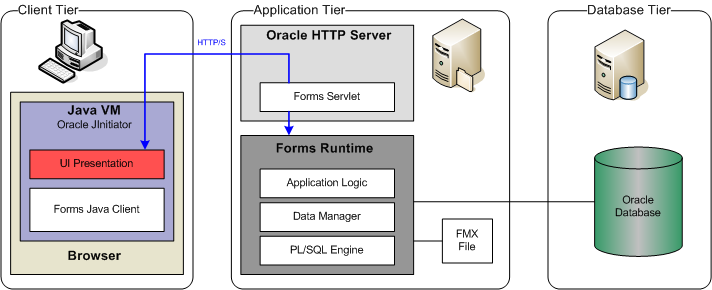
\includegraphics[scale=0.55]{obr/3tier.png}
  \label{}
\end{figure}
TODO zobrazit jako desktop klienta
\subsection{Triggery}
\begin{itemize}
\item Block-processing triggers: - Block processing triggers fire in response to events related to record management in a block.
\item Interface event triggers: - Interface event triggers fire in response to events that occur in the form interface.
\item Master-detail triggers: - Form Builder generates master-detail triggers automatically when you define a master-detail relation between blocks. The default master-detail triggers enforce coordination between records in a detail block and the master record in a master block.
\item Message-handling triggers: - Form Builder automatically issues appropriate error and informational messages in response to runtime events.
\item Navigational triggers: - Navigational triggers fire in response to navigational events.
\item Query-time triggers: - Query-time triggers fire just before and just after the operator or the application executes a query in a block. 
\item Validation triggers: - Validation triggers fire when Form Builder validates data in an item or record.
\end{itemize}

\subsection{LOV}
A List of Values is based on a Record Group. In Oracle Forms, a record group is a query that returns some collection of records. Record groups can be used to populate blocks or LOVs and they can be used in procedures. When the user navigates to an item with an LOV attached to it, the LOV key (F9 in MS Windows) can be pressed to call up the LOV. At that time, the query associated with the record group is executed and the results are displayed in a pop up window. Once the user makes a selection from the list, the value or values are returned to the form and placed in the appropriate fields.

\section{Datový model}
\begin{figure}[H]
  \centering
  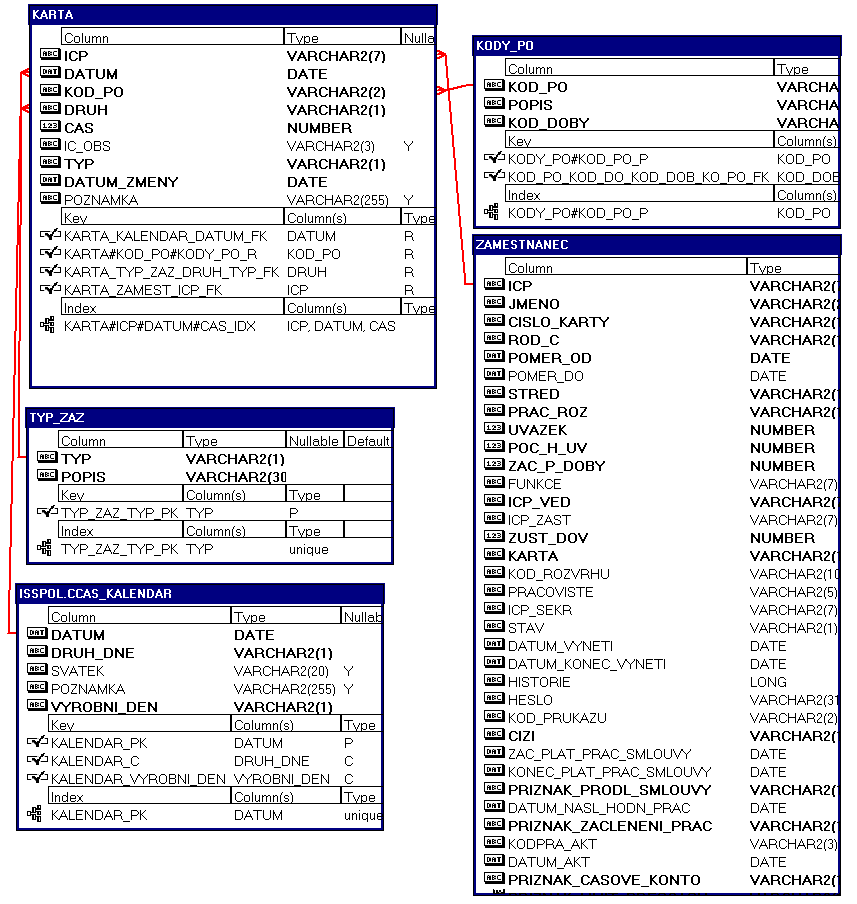
\includegraphics[scale=0.6]{obr/bd27_dochazka.png}
  \label{}
\end{figure}
TODO vytvorit schemata pro datovy model tykajici se jednotlivych modul (dochazka/vykazy), zvyraznit co je vlastne jako podnozina uchovavano na strane android DB

\section{Uživatelské rozhraní}

\subsection{Zápis příchodů a odchodů}
\begin{figure}[H]
  \centering
  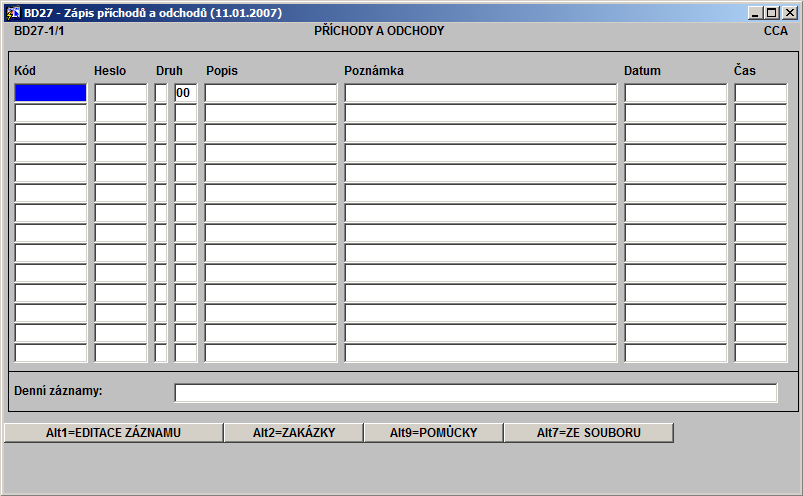
\includegraphics[scale=0.6]{obr/BD27.png}
  \label{}
\end{figure}
+popsat z pohledu uzivatele
\subsection{Výkaz práce}
\begin{figure}[H]
  \centering
  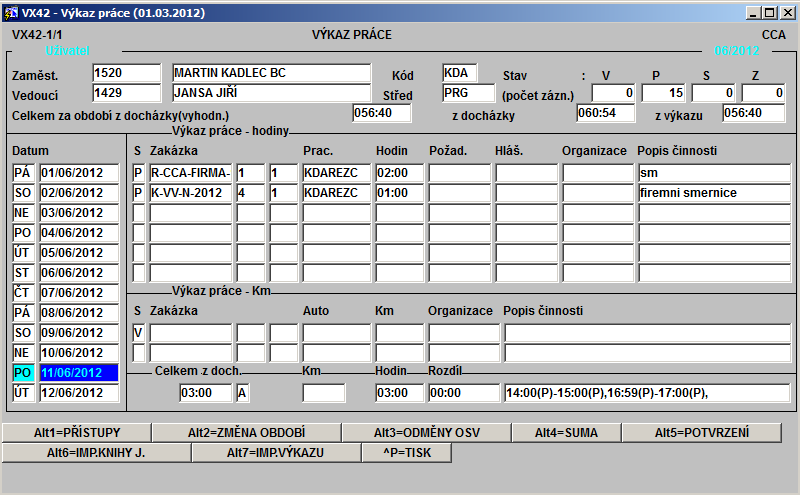
\includegraphics[scale=0.6]{obr/VX42.png}
  \label{}
\end{figure}
+popsat z pohledu uzivatele

\chapter{Analýza}

\section{Architektura}
\subsection{Přímé připojení k databázi}
\subsection{Oracle Database Mobile Server}
Oracle Database Mobile Server 11g - zajistuje synchronizaci mezi Oracle db a mobilnim zarizenim, zamitnuto z licencnich duvodu, mozna by stalo za to to vic prozkoumat a neco o tom napsat
\subsection{Webová služba}

\section{Datová vrstva}
\subsection{Práce s datumem a časem}
Při návrhu datového modelu jsem řešil problém pomocí jakého datového typu vyjadřovat údaj o čase či datu. V Oracle databázi je použit datový typ Date. SQLite databáze nabízí tři způsoby jako ukládat informaci o čase:
\begin{itemize}
\item \textbf{TEXT} podle ISO8601 normy ve formátu "YYYY-MM-DD HH:MM:SS.SSS".
\item \textbf{REAL} podle Juliánského kalendáře, počet dní od poledne 24. Listopadu roku 4714 před kristem (Greenwichského času).
\item \textbf{INTEGER} jako Unix Time, počet sekund 1970-01-01 00:00:00 UTC.
\end{itemize}

\noindent
Pro uložení v SQLite databázi jsem zvolil typ INTEGER. V aplikaci (Android klient, webová služba) jsem se rozhodl reprezentovat časový údaj pomocí primitivního typu long. Měl jsem k tomu řadu dobrých důvodů:
\begin{itemize}
\item odpadá starost s formátem datumu při serializaci a deserializace JSON řetězce
\item snadné porovnávání hodnot pomocí relačních operátorů
\item sníží se počet konverzí v aplikaci (např. pro výpočet pozice pro vykreslení komponenty v UI)
\end{itemize}

Také jsem se ujistil, že rozsah typu long je pro potřeby aplikace dostačující. Srovnání použitých datových typů je znázorněno v tabulce \ref{tab:cas}. 

\begin{table}[H]
\centering
\begin{tabular}{| c | c | c | c |}
\hline
Datový typ &  Minimální hodnota & Maximální hodnota & Přesnost \\ \hline
Oracle Date &   January 1, 4712 BCE  &  December 31, 4712 CE &  sekundy \\ \hline
SQLite INTEGER &    &  &  sekundy \\ \hline
Java long & 2.12.292269055 BC   & 17.8.292278994 AD &  milisekundy \\ \hline
\end{tabular}
\caption{Datové typy reprezentující časový údaj}
\label{tab:cas}
\end{table}

\subsection{Kritika datové vrstvy}
co se mi nelibilo a co bych navrhl jinak a jak, navrh prichody/odchody - jeden radek,
chybi primarni klic - ROWID jako unikatni identifikator, problemy ktere to prinasi,
format casu - problemy s prevodem

\section{Business logika}
existuje někajá možnost převodu formsů do javy - oracle adf - co to je, co to resi, proc to neresi muj problem
\subsection{Triggery}
jen ty, jejichž funkčnost bude muset být implementována.
\begin{itemize}
\item On-Delete, On-Insert, On-Update, Pre-Delete, Pre-Insert, Pre-Update
\item When-Validate-Item
\end{itemize}

\subsection{Databázové balíčky a uložené procedury}

\subsection{Forms knihovny}


\section{Uživatelské rozhraní}
\subsection{LOV}
jaka alternativa v androidu

\chapter{Implementace}

\section{Funkcionalita}
Na základě analýzy současného systému a potřeb zaměstnanců byla vybrána k implementaci následující funkčnost: 
\paragraph{Docházka}
\begin{itemize}
\item Přehledné zobrazení událostí docházky daného zaměstnance
\item Uživatel má možnost přidávat, ediovat a mazat svoje události
\item Aplikace zajišťuje automatickou synchronzaci těchto údajů s firemní databází
\item Zobrazení poměru typů docházkových událostí za dané období
\end{itemize}
\paragraph{Aktuální přítomnost na pracovišti}
\begin{itemize}
\item Zobrazení seznamu zaměstnanců aktuálně přítomných na pracovišti
\item Uživatel má možnost spravovat seznam svých "oblíbených" zaměstnanců a tento seznam zobrazovat přednostně
\end{itemize}
\paragraph{Výkazy práce}
\begin{itemize}
\item Zobrazení poměru typů zakázek za dané období
\item Zobrazení vývoje vývoje daného typu zakázky v daném období 
\item Možnost zobrazení těchto údajů i za jiné zaměstnance
\end{itemize}

\subsection{Nastavení a konfigurovatelnost}
Aplikace si musí pamatovat údaje nutné pro snadnou obsluhu tzn. uživatelské jméno a heslo, adresu umístění webové služby a tyto údaje jsou konfigurovatelné.\\
Dále aplikace umožní uživateli konfigurovat vzhled některých kompoment, jako je barva typu události v docházce a typu záznamu ve výkazech.

\subsection{Uživatelská přívětivost}
Uživatelské rozhraní aplikace klade důraz na přehlednost, ergonomii a časově efektivní obsluhu.

\section{Architektura}
Android aplikace funguje jako tenký klient, který se připojuje k webové službě. Webová služba používá REST architekturu a přistupuje k samotné databázi.

\begin{figure}[H]
  \centering
  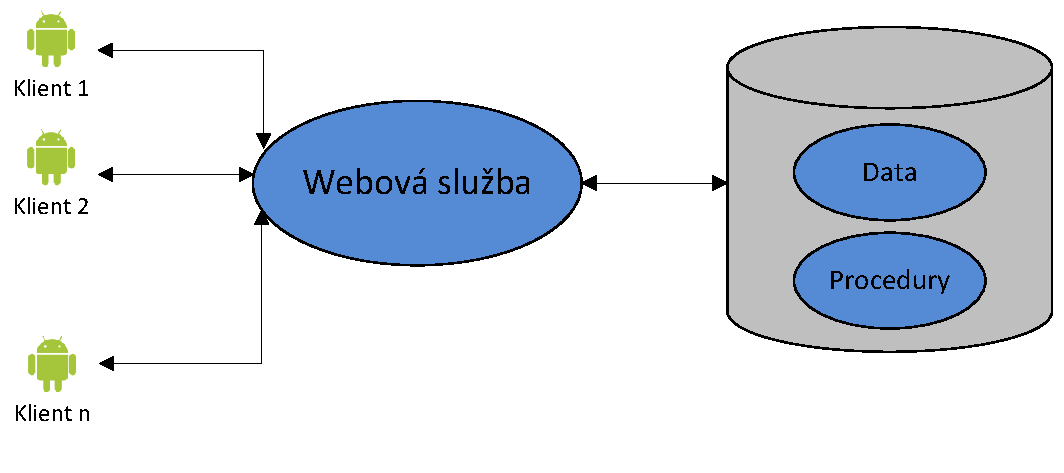
\includegraphics[scale=0.8]{obr/souc_arch2.pdf}
  \label{obr: logo zcu}
\end{figure}

\begin{itemize}
\item Webová služba - Java EE 6, aplikační server GlassFish
\item Databáze - Oracle 10g, obsahuje navíc databázové procedury, které se používají v současných formulářích  
\item Android - obsahuje persistentní úložiště, obsahuje záznamy o docházce, úložiště se bude automaticky synchronizovat ve stavu online s databázovým serverem prostřednictvím webové služby
\end{itemize}
TODO prepsat srozumitelneji
TODO schema komunikace -HHTP, JDBC

\section{Business logika}
prijde to do webove sluzby - duvody

\section{Android komponenty}
\begin{enumerate}
\item komponenty pro sync a auth, provazani s android ucetm
\item CursorLoader
\item Async task
\item  nestandartni UI
\item modifilkace adapterview
\item cutom UI - viewgroup
\end{enumerate}
+ nejaka ukazka konkretniho pouziti

\section{SQLite}
je treba resit delku dat napriklad stringu?, dynamic typing

V knihovnách pro Forms aplikace se nachází další kód, který bude nutné přepsat do webové služby.
\section{REST}
\begin{enumerate}
\item REST operace - davkove vs jednotlive
\item REST, tabulka URI, 
\end{enumerate}

\section{Synchronizace}
\begin{enumerate}
\item sync algoritmus - 2 algoritmy (jeden ideální, druhý reálný), srovnání
\item sync architektura - komponenty
\end{enumerate}

\section{Zabezpečení}
-authentikace
Server webové služby je dostupná v síti VPN. Další zabezpečení bude řešeno později...

\section{Zpětná kompatibilita}

\section{Budoucí rozšiřitelnost}

\section{O čem psát...}
\begin{enumerate}
\item popsat IMIS 
\item pripraveno webove sluzby na dalsi mobilni platformy
\item cinnost apliakce online/offline
\item flow diagramy pro ruzne cinnosti
\item pristupova prava
\item uspora pesistentni pameti na strane androida
\item chybove reporty a opravy na aplikaci v ostrem prostredi, obrazek + ukazka
\item jak zjisit zmenu zaznamu, v datech se uklada pouze datum posledni zmeny, nikoli presny cas
\item perioda automatickeho mazani dat
\end{enumerate}

\appendix
\bibliographystyle{csplainnat}
%\bibliography{bakalarka}
\end{document}
